\documentclass[a4paper,10pt]{problems}

\newcommand{\A}{{\ensuremath{\mathcal{A}}}}
\newcommand{\B}{{\ensuremath{\mathcal{B}}}}
\newcommand{\CC}{{\ensuremath{\mathcal{C}}}}

\begin{document}
\Header{Время работы (сложность) алгоритмов}

\begin{flushright}
Автор: Петр Калинин, основной текст: 2008\\
Этот документ можно распространять по лицензии\\
Creative Commons Attribution-ShareAlike 3.0 Unported (CC BY-SA 3.0)\\
Последнюю версию, а также исходный код для системы \LaTeX\\
можно скачать с \verb`https://github.com/petr-kalinin/progtexts`\\
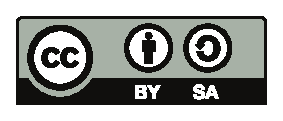
\includegraphics[width=2cm]{by-sa-corr.eps}
\end{flushright}

Пожалуй, одним из основных параметров, по которому вы должны выбирать, подходит 
ли тот или иной алгоритм для решения задачи на олимпиаде (естественно, помимо 
корректности алгоритма) "--- это его время работы, или, как говорят, сложность. 
Когда ещё только собираетесь писать решение, важно верно оценить его сложность 
и определить, уложится ли этот алгоритм в ограничение по времени. Если не 
укладывается, то, возможно, стоит поискать другой или как минимум понимать, что 
ваш алгоритм будет тормозить.

На самом деле половина, если не больше, приведённого текста здесь вам скорее 
для справки, на случай, если в будущем вы будете сталкиваться с упоминанием о сложности и 
использованием $O$-обозначений и не поймёте что-нибудь. В частности, может быть 
поэтому, текст какой-то сумбурный (особенно первая часть) у меня получился.

\header{Примеры и $O$"=обозначение}

\lheader{Пример 1: сложность алгоритма Флойда}
Рассмотрим следующую программу (алгоритм Флойда вычисления кратчайших путей 
между всеми парами вершин в графе, применённый к задаче поиска отрицательных 
циклов в графе, но это пока не важно):
\begin{codesample}\begin{verbatim}
begin
assign(f,'input.txt');reset(f);
read(f,n);
for i:=1 to n do
    for j:=1 to n do
        read(f,w[i,j]);
close(f);
for i:=1 to n do
    for j:=1 to n do
        for k:=1 to n do
            if w[j,k]>w[j,i]+w[i,k] then
               w[j,k]:=w[j,i]+w[i,k];
ok:=false;
for i:=1 to n do
    if w[i,i]<0 then
       ok:=true;
assign(f,'output.txt');rewrite(f);
if ok then
   writeln(f,'Negative cycles exist')
else writeln(f,'No negative cycles');
end.
\end{verbatim}\end{codesample}

Попробуем определить, сколько времени займёт выполнение этой программы. 
Очевидно, что, прежде чем дать точный ответ на этот вопрос, надо решить 
следующие вопросы:
\begin{ulist}
\item Для каких конкретно входных данным мы будем определять время?
\item На каком компьютере будет выполняться программа (в смысле, сколько 
времени займёт выполнение тех или иных операций и т.п.)
\item Возможно, что-то ещё :)
\end{ulist}

Но, с другой стороны, знание точного времени выполнения на конкретном 
компьютере на конкретных входных данных нам не очень-то и нужно, и можно даже 
сказать, что вообще не нужно (мы все равно \textit{точно} не знаем компы жюри, 
не заем тестов, да и все равно точно все оценить не сможем).

Но зато в условии задачи стоит, скорее всего, ограничение на $N$, да и 
понятно, что в первую очередь от $N$, а не от конкретных входных данных,
зависит время работы программы (в смысле, что, если я увеличу $N$ в 10 раз, то 
программа резко затормозится, а если я, например, увеличу вес\'{а} всех, или части, 
рёбер, то время почти не изменится). Кроме того, жюри может оказаться очень 
злобным  
и подсунуть самый противный тест, поэтому мы будем интересоваться в первую 
очередь временем работы программы \textit{в худшем случае среди всех случаев с 
данным $N$}. 

\note{Есть редкие исключения, например, QSort, у которого худшие 
случаи встречаются \textit{очень} редко и, если писать QSort рандомизированно 
(т.е. выбирать всегда не средний, а случайный элемент), то никакое даже очень 
злобное жюри не сможет подобрать неприятный тест. Поэтому для QSort'а 
интересуются в первую очередь \textit{средним} временем работы (по всем 
возможным тестам с данным $N$), а не худшим, которое сильно отличается от
среднего (подробнее далее). Ещё пример "--- хеширование (если вы не знаете, что 
это такое, то не страшно :) ). Но это "--- пожалуй, единственные исключения. 
Обычно, во"=первых, среднее время не очень сильно отличается от худшего, а 
во"=вторых, худший тест подобрать реально, и жюри, скорее всего, постарается 
это сделать.
}

Итак, нам нужно определить время работы этой процедуры в худшем случае, причём 
в первую очередь выделив зависимость от $N$. На самом деле нас удовлетворит 
даже не очень плохая оценка сверху (т.е. сойдёт, если мы приведём функцию, 
которая всегда даёт чуть большее время, чем на самом деле). Так как нам все 
равно неизвестны точные характеристики компьютера, на котором будет 
тестирование, да и мы их все равно не смогли бы учесть, то \textit{абсолютно 
точно} все равно не получится оценить.

Поэтому заметим, что у нас есть действия, которые выполняются 
\textit{фиксированное} число раз, не зависимо от $N$ (например, 
\verb|read(f,n);| и т.п.). Обозначим сумму времён выполнения таких операций (в 
худшем случае) за $A$. Есть операции, которые выполняются за время, примерно 
пропорциональное $N$ (последний цикл, \textit{а также}, в том числе, операции, 
связанные с внешними циклами: увеличение $i$ на единицу, сравнение его с $N$ и 
т.д.; именно работа с $i$, а не с $j$ или с $k$). Обозначим сумму всех таких 
времён в худшем случае (хотя они не сильно зависят от случая) за $BN$ (она 
пропорциональна $N$, поэтому выделим его в отдельный множитель). Аналогично, 
есть команды, которые работают за время, пропорциональное $N^2$ (цикл ввода, 
\textit{а также} работа с $j$: увеличение на единицу, сравнение с $N$ "--- в 
обоих циклах) "--- обозначим сумму времён за $CN^2$ "--- и есть команды, 
работающие за время, пропорциональное $N^3$ (в частности, тот самый внутренний 
\verb|if|, время работы которого действительно зависит от входных данных) "--- 
обозначим сумму времён за $DN^3$.

Общее время работы получается $A+BN+CN^2+DN^3$, причём $A$, $B$, $C$ и $D$ 
здесь некоторые константы, которые, конечно, зависят от компьютера, для 
которого мы пишем время, но \textit{не зависят} ни от $N$, ни даже от 
конкретного теста при данном $N$ (т.к. мы все суммировали для худшего случая). 
Заметим, что точнее этой формулы вряд ли мы сможем что-нибудь сказать, т.к. все 
равно не знаем и не можем учесть характеристик компьютера. Кроме того, обычно 
все-таки величины $A$, $B$, $C$ и $D$ не сильно отличаются друг от друга (ну, 
максимум раз в десять :) ), а даже при $N$ равном 100 получается, что $N^2$ 
отличается от $N$ в сто раз, и аналогично $N^3$ от $N^2$. Ещё хуже будет, если 
$N$ будет ещё больше. Проще говоря, $DN^3\gg CN^2\gg BN \gg A$, причём чем $N$ 
больше, тем эти соотношения выполняются лучше (символ $\gg$ обозначает "<много 
больше">, как минимум в несколько раз; точные критерии того, что есть много 
больше, зависят от ситуации,  
конечно). Поэтому в выражении для времени выполнения можно оставить только 
старшее слагаемое: $DN^3$, все равно остальные намного меньше его, и потому 
результат изменят не сильно (ну и пусть остальные увеличат результат на 10\% 
"--- все равно мы точно не знаем $D$, и все равно нам такая точность не нужна). 
Более того, можно выбрать $\delta$ такое, чтобы $\delta N^3$ было всегда 
больше, чем $A+BN+CN^2$ (см. подробнее ниже), и тогда, заменив $D$ на 
$D'=D+\delta$, можно гарантировать, что $D'N^3$ будет \textit{всегда} больше 
времени выполнения программы. Т.е. мы нашли неплохую оценку сверху (она 
отличается от правильного времени не очень сильно).

Итак, время работы нашей программы можно неплохо оценить как $DN^3$, и лучше 
этого мы все равно ничего не получим. Но $D$ мы все равно не знаем. Поэтому 
можно говорить, что наша программа работает \textit{за кубическое время}, за 
время, \textit{пропорциональное} $N^3$, не забывая про наличие неизвестного нам 
постоянного множителя. Поэтому при оценке сложностей алгоритмов часто 
используется $O$"=обозначение.

\lheader{$O$"=обозначение}
Пусть у нас есть две функции $f(n)$ и $g(n)$, и пусть существуют такая (не зависящая от $n$) константа $\alpha$, что 
$f(n)\leq \alpha g(n)$ при любых $n$, начиная с некоторого. Тогда говорят, что \textit{$f(n)$ есть 
O"=большое от $g(n)$} (или, короче, О от $g(n)$), и пишут, что $f(n)=O(g(n))$. Замечу, 
что условие $f(n)\leq \alpha g(n)$ начиная с некоторых $n$, равносильно условию, что $f(n)/g(n)$ не 
превосходит некоторой константы, начиная с некоторых $n$.

\iffalse
\note{Иногда дают другое определение: $f(n)=O(g(n))$, если существуют \textit{две} 
константы $\alpha _1$ и $\alpha _2$ такие, что $\alpha _1g(n)\hm\leq f(n)\hm\leq \alpha _2g(n)$, начиная с некоторых $n$. 
Эти два определения \textit{не} равносильны: например, в соответствии с первым определением, 
$n^2=O(n^3)$, т.к., начиная с $n=1$ (т.е. при любых $n\geq 1$) имеем, что $n^2/n^3\leq \alpha $, 
если взять $\alpha $, например, равным 1. В соответствии же со вторым определением $n^2\neq O(n^3)$. 
Я далее буду придерживаться первого определения, ниже поясню, почему.

Кроме того, иногда вводят ещё множество различных обозначений типа $\Theta(g(n))$, 
$\Omega(g(n))$, вообще говоря, ещё и $o(g(n))$ (причём $o$ (о-малое) и $O$ (о-большое) "--- это 
весьма разные вещи), если хотите посмотреть поподробнее, то смотрите в Кормене, но имхо обычно 
это все (кроме $O$"=обозначения) не очень надо.}
\fi

С использованием $O$"=обозначения сложность программы в первом примере можно записать как 
$O(N^3)$. Действительно, очевидно, что
$$
{AN^3+BN^2+CN+D\over N^3}=A+{B\over N}+{C\over N^2}+{D\over N^3}\leq (A+B+C+D) \qquad\mbox{при $N\geq1$}, 
$$
поэтому взяв $\alpha=(A+B+C+D)$, мы точно обеспечим выполнение нужного условия. 

\note{Более того, можно взять $\alpha=A+B/10+C/100+D/1000$, и условие будет выполнено при 
$N\geq 10$, можно взять $\alpha=A+B/100+C/10^4+D/10^6$, и условие все равно будет выполнено 
при любом $N\geq 100$ и т.""д. "--- поэтому видно, что константа $A$ важнее 
всех остальных.}

Вообще, аналогично можно показать, что для любого полинома $P(n)$ степени $k$ (т.е. 
$P(n)\hm=a_kn^k\hm+\dots\hm+a_1n+a_0$) верно, что $P(n)=O(n^k)$, и наиболее важным коэффициентом 
является $a_n$.

$O$"=обозначение почти всегда является очень удобным для обозначения сложности работы алгоритмов. 
Действительно, как мы видели, \textit{абсолютно точно} оценить время работы программы 
невозможно, да и не нужно. Самое лучшее, что мы можем сделать "--- это определить выражение с 
точностью до некоторого более-менее постоянного множителя, а $O$"=обозначение как раз и есть 
то, что сохранит этот результат и скроет все не важные нам подробности. Кроме того, определять 
сложность алгоритмов именно в смысле $O$"=обозначения как правило очень легко, примеры см. 
ниже.

$O$"=обозначение скрывает константу, поэтому если есть две функции $g(n)$ и $h(n)$, которые 
отличаются в константу раз, т.е. $g(n)/h(n)$ не зависит от $n$, то $O(g(n))$ и 
$O(h(n))$ "--- это одно и то же. Например, $O(n)$, $O(2n)$, $O(10n)$ и 
$O(3.14n)$ на самом деле обозначает одно и то же.

Как показывает опыт, на 
современных компьютерах при современных ограничениях по времени программа уложится в 
ограничение по времени, если ей нужно будет сделать примерно 100 миллионов "<действий">. 
Поэтому для довольно грубой оценки того, подходит ли тот или иной алгоритм, можно проверять, 
укладываетесь ли вы в это ограничение. А именно, если, например, сложность программы $O(n^3)$, 
то она обычно уложится во время при $n$, не превосходящем 400--500, если сложность $O(n^2)$ 
"--- то при $n$, не превосходящем $8\,000$--$15\,000$, и т.д. (в этом смысле выше я и взял 
слово "<действий"> в кавычки: поскольку все равно все оценки приблизительные, то можно просто 
подставить $n$ в формулу, стоящую под знаком $O$, и проверить, что получится).

Это и есть \textbf{основное практические применение $O$-обозначений на олимпиадах}. Чтобы оценить, 
укладывается ли ваше решение в ограничение по времени, подставляете максимальное $n$ в сложность 
алгоритма, и если результат получается существенно меньше $10^8$, то скорее всего укладывается, если 
существенно больше чем $10^8$ (грубо говоря, больше чем $10^9$), то вряд ли, иначе у вас пороговый 
случай и придется смотреть внимательнее. В последнем случае уже становится важна константа: если 
"<действия"> вашей программы простые (сложения/умножения целых чисел), то ограничение по $n$ можно 
и увеличить, если же сложные (деление целых чисел, действия с веществеными числами и т.д.), но 
нельзя.

$O$"=обозначение указывает на самом деле на поведение функции $f(n)$ при больших $n$, в этом 
смысле часто $g(n)$ называют \textit{асимптотикой} для $f(n)$. 

Особого упоминания заслуживает обозначение $O(1)$. Это обозначает (в соответствии с 
определением выше), что функция $f(n)$ не растёт с увеличением $n$, что есть некоторая не 
зависящая от $n$ константа, ограничивающая $f(n)$ сверху: $f(n)\leq \alpha$. Поэтому 
в некотором смысле это обозначает, что время работы не зависит от $n$ (конечно, оно может 
зависеть, но оно не стремится к бесконечности с увеличением $n$). На самом деле тот же смысл 
имеет обозначение $O(2)$ и т.п., но обычно принять писать $O(1)$ (точно также как $O(2n)$, 
$O(n)$, $O(3.14n)$ и т.п. на самом деле все одно и то же, но пишут обычно $O(n)$ и т.п.).

Ещё замечу, что само по себе обозначение $O(g(n))$ имеет не до конца понятный смысл. Чёткий 
смысл имеет обозначение `$=O(g(n))$', т.е. вместе с знаком равенства, а без него не ясно, что 
такое $O(g(n))$. Например, я могу написать $O(n)+O(n^2)$, но что это значит, нужно уточнять 
особо. Если тут вроде все-таки все более-менее понятно (сумма двух функций, первая из которых 
\textit{есть} $O(n)$, а вторая "--- $O(n^2)$), то если я запишу, например,
$$
\sum_{i=1}^{n} O(i),
$$
то здесь все-таки хочется дополнительных пояснений. Конечно, может быть, можно определить 
$O$"=обозначение так, чтобы оно и тут давало однозначную трактовку, но лучше не употреблять $O$ 
вообще нигде, кроме как в правой части равенств в формате `$=O(g(n))$' (или в выражениях типа 
"<время выполнения составляет $O(g(n))$">, что подразумевает, что $T(n)=O(g(n))$, где $T(n)$ 
"--- время выполнения, в худшем случае, например).

Ещё замечу, что $O$"=обозначение, как следует из его определения, вполне может 
использоваться и для других случаев, не только для описания времени работы 
программы. Например, нередко оно используется для указания количества \textit{памяти}, 
используемой программой: опять"=таки, чтобы не указывать \textit{сколько вешать 
точно в байтах}, а указать порядок: например, правильное решение некоторой задачи 
требует всего $O(M)$ памяти. Ещё пример на употребление $O$"=обозначения не для указания времени работы программы: пусть мы говорим, что какая-нибудь программа требует $O(N\log N)$ 
операций с длинными числами "--- тогда это не есть сложность (время выполнения) 
программы, т.к. операции с длинными числами работают не за $O(1)$ (!), но тем не менее это даёт определённую информацию о времени выполнения. 
Ещё пример (который будет употребляться ниже): размер входного файла в 
какой-нибудь задаче есть $O(N^2)$.

\lheader{Ещё примеры}

\begin{codesample}\begin{verbatim}
for i:=1 to n do
    for j:=i+1 to n do begin
        ...
    end;
\end{verbatim}\end{codesample}
Общее количество выполнения внутренней части цикла будет 
$(n-1)+(n-2)+\dots+2+1\hm=n(n-1)/2\hm=n^2/2-n/2\hm=O(n^2)$, т.к. выражение является полиномом второй 
степени. Очевидно, что время выполнения всех остальных операций в этом цикле будет не больше, 
чем $O(n^2)$, поэтому время выполнения всего этого куска кода будет $O(n^2)$. (Конечно, здесь 
и далее я считаю, что внутренний кусок кода, заменённый на \texttt{...}, выполняется за 
$O(1)$).

\begin{codesample}\begin{verbatim}
for i:=1 to n do
    for j:=i+1 to n do
        for k:=j+1 to n do
            for l:=k+1 to n do begin
                ...
            end;
\end{verbatim}\end{codesample}
Точную формулу количества операций получить, может быть, нетривиально, но ясно, 
что будет полином четвёртой степени, поэтому все равно $O(n^4)$. Конечно, такая 
программа работает быстрее, чем если бы все циклы были от 1 до $n$, но на асимптотику это не влияет (см. ещё ниже).

\begin{codesampleo}\begin{verbatim}
for i:=1 to n do
    for j:=1 to round(sqrt(n)) do
        ...
\end{verbatim}\end{codesampleo}
Сложность $O(n\sqrt{n})$. На самом деле корни в сложности встречаются нечасто, обычно только 
во всяких задачах на проверку чисел на простоту, а также в условно называемой эвристике 
$\sqrt{n}$. Обратите также внимание, что всякие округления 
делать тут не надо: ну и что, что $\sqrt n$ может не быть целым. У нас все равно везде стоят 
\textit{не}равенства, да ещё есть произвол в выборе $\alpha$, поэтому беспокоиться об 
округлении тут не надо.

\begin{codesampleo}\begin{verbatim}
for i:=1 to n do begin
    j:=1;
    while j*j<n do begin
          ...
          inc(j);
    end;
\end{verbatim}\end{codesampleo}
Абсолютно аналогично предыдущему.

\begin{codesampleo}\begin{verbatim}
while n>0 do begin
      ...
      n:=n div 2;
end;
\end{verbatim}\end{codesampleo}
Количество итераций цикла будет $\log_2 n$ плюс-минус несколько. 
Поэтому сложность $O(\log n)$. Замечу, что, как известно (может, вы и не 
знаете, но все равно это так) логарифмы по разным основаниям отличаются в 
константу раз, т.е. для любых $a$ и $b$ отношение $\log_a n/\log_b n$ равно 
$\log_a b$ и \textit{не} зависит от $n$, поэтому $O(\log_a n)$ и $O(\log_b n)$ 
на самом деле одно и то же (точно также, как $O(n)$ и $O(2n)$ "--- это одно и 
то же). Поэтому, когда логарифмы попадаются под $O$"=обозначением, основание 
как правило не указывают.

\begin{codesampleo}\begin{verbatim}
for i:=1 to n do ...
for i:=1 to m do ...
\end{verbatim}\end{codesampleo}
Т.""е. два последовательных цикла, один до $n$, второй до $m$. Пока мы не знаем 
соотношения на $n$ и $m$, будем считать, что это просто два отдельных параметра 
задачи. В таком случае нас интересует уже время выполнения как функция 
$T(n,m)$, а не $T(n)$, как было раньше. Поэтому и под символом $O$ у нас теперь 
будут два параметра. Время выполнения этого фрагмента можно считать равным 
$T(n,m)=An+Bm$ при некоторых $A$ и $B$, и обозначив $C=\max(A,B)$, получим 
$T(n,m)\leq C(n+m)$, значит, можно написать $T(n,m)=O(n+m)$. Время выполнения 
этого куска есть $O(n+m)$. Вообще, иногда бывает так, что есть несколько, а не один, 
параметр, зависимость от которых нас интересует (самый, пожалуй, частый пример 
"--- алгоритмы на графах: в них, как правило, есть два параметра: число вершин 
$V$ и число рёбер $E$). В таком случае нередко под $O$"=обозначением записана 
\textit{сумма} некоторых выражений. Это обычно имеет как раз смысл, аналогичный 
указанному здесь.

\note{Заметим, что, вообще говоря, приведённое выше определение применить на 
случай функции нескольких переменных в лоб не получится, но несложно его 
модифицировать так, чтобы все стало хорошо. Я делать этого здесь не буду, 
надуюсь, что идея более"=менее понятна, а детали реализации определения все 
равно не очень важны "--- строго надо бы немного по"=другому писать все равно.}

\lheader{Последовательность сложностей} Все возможные асимптотики можно 
упорядочить от более быстрых к более медленным. Получится примерно следующее:
$\log n$, $\log^2 n$, $\sqrt[3]{n}$, $\sqrt{n}$, $n$, $n\log n$, 
$n\log^2n$, $n\sqrt n$, $n^2$, $n^3$. (естественно, между каждыми членами этой 
последовательности можно вставить ещё сколько угодно асимптотик, потому, в 
частности, я не пишу тут нигде многоточий).

Т.е.: все логарифмы идут в порядке увеличения степени, все степени $n$ 
($\sqrt n=n^{1/2}$, $n=n^1$, $n^2$ и т.п.) идут в порядке увеличения степени, 
\textit{любая} степень логарифма идёт \textit{до} любой степени $n$ (в 
частности, $\log^{100} n$ идёт \textit{до} $\sqrt[100] n$);  
соответственно, $n\log^k n$ при любом $k$ идёт до $n^{1+\eps}$ при любом 
$\eps>0$ и т.п.

\header{Дополнительные замечания}
\lheader{Сложность переборных решений} В отличии от нерекурсивных решений, сложность 
рекурсивных решений оценить обычно очень нетривиально, а в случае с переборными 
решениями ещё и, как правило, не нужно (в частности, потому я и 
решил, что тему про перебор можно давать \textit{до} темы про сложность). Очень 
грубо время работы переборного решения можно оценить по количеству листов в дереве перебора (и 
именно это количество, т.е. количество перебираемых вариантов, и стоит 
сравнивать с величиной 1--100 миллионов), но это, 
может быть, даже не будет асимптотикой. Ближе к асимптотике будет подсчёт 
\textit{общего числа} узлов в дереве, а может, ещё стоит умножить на количество 
итераций всяких циклов, которые, может быть, присутствуют в процедуре find. Но, 
с другой стороны, считать асимптотику (т.е. использовать $O$"=обозначение) для 
переборных решений все равно бессмысленно, т.к., во-первых, при маленьких $n$ 
асимптотика довольно бессмысленна (она приобретает смысл, т.е. соответствие 
реальности, при больших $n$, а в задачах на перебор $n$ обычно мало), а 
во"=вторых, очень сложно оценить действие различных эвристик и отсечений. 
Поэтому $O$"=обозначение для переборных решений обычно не используется. 

\note{Кстати, обратите внимание, что $3^n\neq O(2^n)$, соответственно 
$2^{2n}\neq O(2^n)$ и т.п.}

\lheader{Про QSort подробнее} Несложно видеть, что в худшем случае сложность 
QSort'а есть $O(n^2)$: если на каждом шагу QSort будет отщеплять один-два 
элемента, то глубина рекурсии будет $O(n)$, каждый уровень рекурсии выполняется 
за время порядка $O(r-l)$, где $r$ и $l$ "--- границы диапазона, итого порядка 
$1+2+\dots+n\hm=O(n^2)$. Но можно показать, что \textit{в среднем} по всем 
тестам с данным $n$  сложность работы QSort'а будет $O(n \log n)$. Конечно, 
если каждый раз брать вполне определённый элемент в качестве разделяющего 
(например, всегда первый, или всегда средний), то несложно будет злобному жюри 
подобрать тест, на котором ваша программа будет работать за $O(n^2)$. Но, 
если на каждом шагу выбирать разделяющий элемент случайно, то никакое злобное 
жюри не сможет ничего поделать.

\lheader{О константе} Как мы видели, $O$"=обозначение скрывает константу 
пропорциональности: если мы пишем, что время $O(n)$, то это значит, что при 
больших $n$ время примерно пропорционально $n$, но коэффициент 
пропорциональности (константу) мы не указываем. И 
логично: абсолютное значение константы нам не нужно: все равно мы его точно 
определить не можем. Но если у нас есть \textit{два} алгоритма, то может иметь 
смысл \textit{сравнить} их константы. Как правило, все равно алгоритм с худшей 
сложностью будет проигрывать по времени, но при равных асимптотиках иногда имеет 
смысл оптимизировать константы, да и иногда алгоритм с меньшей константой, но 
большей асимптотикой при конечных $n$ (какие и бывают в задачах) может обходить 
алгоритм алгоритм с большей константой, но меньшей асимптотикой.

В общем, оптимизировать константу все равно стоит, хотя и во вторую очередь (в 
первую очередь оптимизируйте сложность!), особенно если оптимизировать 
константу ничего не стоит. Например, пишите \texttt{for i:=1 to n do for j:=i+1 to 
n do} вместо \texttt{for i:=1 to n do for j:=1 to n do}, где это можно.

\lheader{Сложные случаи} Далеко не у всех решений сложность 
оценивается так легко, как это было в предыдущих примерах. Например, рассмотрим 
следующую программу (найти четыре одинаковых числа в массиве):
\begin{codesample}\begin{verbatim}
for i:=1 to n do 
    for j:=i+1 to n do if a[i]=a[j] then
        for k:=j+1 to n do if a[i]=a[k] then
            for l:=k+1 to n do if a[i]=a[l] then begin
                вывести решение;
                halt;
            end;
\end{verbatim}\end{codesample}
Если бы не было команды \texttt{halt;}, то вопросов не было бы: сложность 
$O(n^4)$ и TL на тестах, в которых много одинаковых чисел. Но \texttt{halt;}, видимо, 
меняет сложность до $O(n^2)$. Действительно, если длины все числа разные
разные, то в первый же \texttt{if} программа никогда не войдёт, и внутренние циклы работать не будут. Если же много одинаковых 
чисел, то очень быстро найдётся решение и будет \texttt{halt;} (правда, строго 
доказывать, что сложность $O(n^2)$, я не умею, но вроде правдоподобно).

\note{Есть известная история про белорусскую команду на межнаре'2002. Там была 
задача, в которой было очевидное решение за $O(n^3)$ (что не укладывалось во 
время), и никто из наших (в т.""ч. я) и не придумали, что его можно легко 
улучшить до $O(n^2)$, и потому придумывали разные хитрости. А белорусы, не придумав ничего 
лучше, написали этот алгоритм, но с небольшим улучшением. После тура они нам 
сказали, что не смогли придумать тест, на котором бы их решение тормозило, но и
не смогли доказать, что такого теста нет. Мы тоже долго думали, но тоже не
придумали. А потом прочитали официальное решение и поняли, что оно фактически
представляет собой \textit{доказательство} того, что белорусское решение работает за
$O(n^2)$.}

\header{Классы $P$ и $NP$. $NP$-полнота}

Теория классов сложности $P$ и $NP$ имхо весьма интересна сама по себе, а кроме 
того, нередко бывает полезна на практике, чего от такой, на первый взгляд, 
весьма теоретизированной теории как"=то и не ожидаешь :). Кроме того, она 
приводит к, пожалуй, самой известной ещё пока неразрешённой проблеме 
программирования: верно ли, что $P=NP$? Поэтому имхо полезно это все 
себе представлять, тем более что в дальнейшем я, наверное, буду иногда ссылаться на 
этот материал. С другой стороны, если вы не поймёте это с первого раза, тоже не 
страшно. Может быть, вы не поймёте какую-то часть "--- попробуйте читать 
дальше, вдруг вы поймёте дальнейшие идеи.

Материал, по-моему, весьма неплохо изложен в Кормене. Большинство определений, 
которые я даю тут, не до конца строгие; более строго это, наверное, изложено в 
Кормене.

\lheader{Естественный параметр теста} Везде раньше у нас было довольно ясно, 
функцией от чего должна быть сложность: везде под $O$"=обозначением стояла 
некое число $n$, которое, как подразумевалось, достаточно хорошо характеризует 
размер теста. Но с другой стороны ясно, что в выборе $n$ как параметра теста 
есть довольно широкий произвол; более того, могут быть ситуации, когда далеко 
не очевидно, чт\'{о} именно будет служить хорошим параметром теста; более того, 
иногда хочется ввести несколько таких параметров сразу и т.""п. Короче говоря, 
если мы хотим строить какую"=то более"=менее универсальную теорию, 
классифицирующую алгоритмы по сложности и т.п., то надо иметь какой"=то 
более"=менее универсальный, естественный, способ выбора параметра теста, т.е. 
того, что будет стоять под $O$"=обозначением, чтобы не думать каждый раз.

Таким весьма удобным параметром можно выбрать размер входного файла, который 
везде далее будем обозначать $L$ (точнее, везде далее $L$ будет обозначать 
размер входного файла), и сложность мы будем мерить именно как функцию от $L$. 
Это на первый взгляд несколько неудобно, т.к. обычно в условии задачи стоит 
ограничение не на размер файла, а на какое-нибудь $N$, но, как мы увидим далее, 
в большинстве разумных случаев класс алгоритма останется тем же, даже если 
сложность мы запишем как функцию $N$; как функцию $L$ мы её будем записывать 
лишь затем, чтобы избавиться от этих слов "<в большинстве \textit{разумных} 
случаев">.

\lheader{Полиномиальные алгоритмы и класс сложности $P$} Про функцию 
$f(m)$ можно говорить, что она \textit{полиномиальна} по $m$, если она есть 
$O(m^k)$ при некотором $k$. В частности,
\textit{полиномиальным} называется такой алгоритм, сложность которого есть 
$O(L^k)$ при некотором фиксированном $k$. Это обозначает, что его сложность 
является полиномом (т.е. многочленом) от $L$ (или ещё более быстрой функцией, 
например, логарифмом $L$).

Соответственно, класс задач, имеющих полиномиальное решение, называется 
\textit{классом $P$} (слово "<класс"> очень часть используется как синоним слова 
"<множество">).

\note{Если мы хотим расклассифицировать алгоритмы на "<быстрые"> и "<медленные">, то 
в первом приближении логично полиномиальные алгоритмы считать "<быстрыми">, а 
остальные "--- медленными. Логично: ведь, например, разница во времени выполнения 
программы $O(n)$ и $O(n^{10})$ при больших $n$ будет намного менее существенна, 
чем между $O(n^{10})$ и $O(2^n)$. Поэтому вся идеология классов $P$ и $NP$ 
подразумевает в некотором смысле, что полиномиальные алгоритмы "--- это быстрые 
алгоритмы и их можно реализовать и дождаться результата работы, а остальные 
алгоритмы намного медленнее и, грубо говоря, не всегда хочется ждать результата 
их работы. Ещё раз, это скорее идеология, которая лежит под всеми нижеидущими 
определениями, т.е. это просто объяснения, почему все определения даются именно 
так.
}

\note{Заметьте, что, в соответствии с \textit{нашим} определением, $\log 
n=O(n)$ и т.п.}

\note{Замечу, что в \textit{большинстве разумных случаев} размер входного файла есть 
полином (здесь именно полином, а не логарифм и т.п.!) от какого-нибудь параметра
$n$, указываемого в условии задачи (например, в задачах на граф размер входного
файла есть обычно $O(n^2)$, где $n$ "--- количество вершин в графе). В таких
случаях полиномиальный алгоритм имеет также сложность $O(n^{k'})$ при некотором
$k'$ (возможно, не равным $k$), где $n$ "--- некоторый параметр теста из условия
задачи, и потому вместо $L$ в определении полиномиальности можно использовать
$n$. Тем не менее, это не всегда так просто. Например, в задачах длинной
арифметики алгоритм, работающий за $O(n)$, где $n$ --- одно из таких длинных
чисел, нам, как правило, не интересен. Там логичнее использовать в качестве
параметра теста \textit{количество цифр} в числах (обозначим его $m$), а не сами
числа, т.""е. фактически логарифмы чисел. В таком случае размер входного файла
будет полиномиальным по $m$, и $m$ полиномиально по $L$, и полиномиальный по $L$ 
алгоритм будет полиномиальным и по $m$ и наоборот.}


\lheader{Сводимость задач} Пусть у нас есть две задачи, \A{}  и \B. Попробуем 
решить задачу \A{} с помощью решения задачи \B. А именно, пусть у нас есть 
некоторое решение задачи \B{} "--- программа (exe-шник). Эту программу будем считать 
"<чёрным ящиком"> в том смысле, что мы не будем лезть в её внутреннее устройство, а будем её использовать лишь подавая некоторые данные на вход и изучая, что же она выдаст на выходе. Попробуем с 
её использованием написать программу решения задачи \A, а именно, попробуем написать 
программу решения задачи \A{} следующим образом: она будет читать входные данные, 
по ним каким"=нибудь (может быть, нетривиальным) образом формировать входной 
файл для задачи \B, потом запускать exe"=шник"=решение задачи \B{}, подсунув ему
сформированный входной файл, потом читать полученный выходной файл и 
формировать по нему свой выходной файл. Т.""е. основная наша задача "--- 
написать два алгоритма: как входной файл к задаче \A{} превратить во входной файл 
к задаче \B, и как выходной от задачи \B{} превратить в выходной файл от задачи 
\A{} (естественно, так, чтобы все это работало корректно, т.е. для любого 
допустимого входного файла задачи \A{} в итоге получался правильный выходной файл задачи 
\A; естественно, мы считаем, что программа"=решение задачи \B{} работает 
корректно). 

Пусть мы сумели придумать эти два алгоритма так, что \textit{оба} они работают 
за полиномиальное время от $L_A$ "--- размера входного файла задачи $A$ (в 
частности, это обозначает, что сформированный входной файл к задаче \B{} будет 
иметь полиномиальный от $L_A$ размер). Тогда говорят, что задача \A{} 
\textit{сводится} к задаче \B. (При этом важно только время работы "<сводящих"> 
алгоритмов, время работы самой программы"=решения \B{} не важно, не важно даже, 
умеем ли мы её решать).

\note{Насколько я понимаю, это есть классическое определение сводимости задач. 
Можно поставить вопрос, можно ли разрешить запускать программу \B{} несколько 
раз, и т.""п., но для дальнейшего это нам будет не важно; мы будем 
придерживаться приведённого выше определения.}

Пример: рассмотрим две задачи: задачу поиска в произвольном графе гамильтонова 
цикла, т.е. цикла, проходящего по каждой вершине ровно один раз, и так 
называемую "<задачу коммивояжёра">: задачу поиска в \textit{полном взвешенном} 
графе минимального по весу гамильтонового цикла (очевидно, что гамильтоновых циклов 
там полно: граф"=то полный :) ). Тогда первая задача сводится ко второй: 
действительно, по входному графу $G$ задачи о гамильтоновом цикле сформируем 
входной граф к задаче коммивояжёра следующим образом: вершин в нем будет столько же, (граф, 
конечно же, будет полным), а ребро между вершинами будет иметь вес 0, если оно 
присутствует в исходном графе $G$, и вес 1, если отсутствует. После этого 
запустим программу"=решение задачи коммивояжёра и, когда она найдёт гамильтонов 
цикл наименьшего веса, проверим, что его вес равен 0. Если равен, то это "--- 
гамильтонов цикл в графе $G$, иначе в графе $G$ гамильтонового цикла не 
существует. (Если же программа"=решение задачи коммивояжёра требует 
неотрицательности рёбер (вдруг), то сделаем веса равными 1 или 2 и будем 
проверять, что вес найденного цикла равен $N$ "--- количеству вершин).

\task|\textit{Эйлеровым} циклом в графе называется цикл, 
который проходит по каждому ребру ровно один раз. Что вы можете сказать о 
задаче поиска минимального по весу эйлерова цикла в полном взвешенном графе? 
Сводится ли к ней задача поиска (какого"=нибудь) эйлерова цикла в произвольном 
графе, и, если сводится, то как?
||Конечно, искать эйлеров цикл минимального веса в 
полном взвешенном графе есть совершенно бессмысленное занятие "--- они там все 
одинакового веса :). Сведение одной задачи к другой аналогично сведению этих 
задач для гамильтонова цикла не пройдёт, но задачи все"=таки сводятся друг к другу, 
просто потому, что обе задачи есть $P$"=задачи.
|||


Заметим, что, в соответствии с этим определением, \textit{любая} $P$"=задача 
сводится к любой вообще задаче. Действительно, сводящий алгоритм будет просто решать задачу 
\A, не обращая внимание на результат работы программы \B{} (ну, при желании, 
для выполнения формальностей определения, подсунув ей какой"=нибудь тест и не 
обращая внимания на результат её работы).

Ещё обратите внимание, что, если задача \A{} сводится к \B, а \B{} в свою 
очередь сводится к \CC, то из этого следует, что \A{} сводится к \CC{} (это 
свойство называется \textit{транзитивностью}).

\note{То, что задача \A{} сводится к задаче \B, обозначает, что задача \A{} в 
некотором смысле \textit{не сложнее} задачи \B. Именно \textit{не сложнее}, 
т.е. может быть и проще. Т.""е., если вы свели задачу \A{} к задаче \B, то это 
обозначает, что любое решение задачи \B{} вы можете применить к решению задачи 
\A, но это \textit{вовсе не обозначает}, что у задачи \A{} нет других, может 
быть, ещё более лучших решений. Возможно, у задачи \A{} есть какие"=то особенности, которые можно использовать в более лёгком и простом алгоритме. Несколько примеров на это я приведу ниже, в предпоследнем параграфе этой темы.
 
А сейчас я приведу пример на несколько более общую идею: если вы смогли придумать, как задачу \A{} решать с помощью задачи \B{} (не 
обязательно \textit{свели} \A{} к \B{} в смысле вышеприведённого определения: может 
быть, сведение у вас получилось неполиномиальным или, наоборот, очень быстрым, и 
вы этим гордитесь :) ), и применили самое лучшее решение задачи \B, то это все равно не 
обозначает, что вы нашли лучшее решение задачи \A. Этот пример не 
непосредственно на то, о чем я только что говорил: здесь все полиномиально и 
потому в рамках приведённого выше определения сводимости все тут благополучно 
сводится ко всему, но зато тут разные сложности. 

Итак, пример. Задача A про муравьёв с NEERC'2007. На плоскости даны $N$ 
белых и $N$ чёрных точек. Требуется каждую белую точку соединить отрезком с 
какой-нибудь чёрной так, чтобы каждая чёрная оказалась соединена ровно с одной 
белой и так, чтобы проведанные отрезки не пересекались. Никакие три точки не 
лежат на одной прямой. Официальное решение, насколько я понял, было следующее: 
рассмотрим немного другую задачу: соединить попарно (чёрную с белой, как и в 
оригинальной задаче) точки так, чтобы суммарная длина проведённых отрезков была 
минимальна. Несложно доказать, что в решении этой задачи отрезки не будут 
пересекаться, т.е. решение второй задачи есть одновременно и решение первой. 
Вторая же задача есть по сути частный случай так называемой задачи о 
назначениях "--- задачи поиска в полном взвешенном двудольном графе полного 
паросочетания минимального суммарного веса. Есть стандартное известное её 
решение, так называемый венгерский алгоритм. Он весьма нетривиален идейно, но 
реализуется за $O(N^4)$ с небольшой константой довольно легко, особенно если 
иметь навык его реализации; его можно реализовать и за $O(N^3)$. Под стать такому положению дел было дано ограничение в 
задаче: $N\leq 100$, что, наверное, позволяло пройти и венгерскому алгоритму за 
$O(N^4)$. Но! На самом деле в этой задаче есть другое решение, которое идейно 
много проще венгерского алгоритма, и легко реализуется за $O(N^3)$, а, 
если немного подумать, то и за $O(N^2 \log N)$. Это решение намного проще, не 
требует знания никаких нетривиальных алгоритмов (типа венгерского), и пишется 
имхо намного легче, но \textit{очень существенно} использует геометрическую 
природу задачи (т.е. использует геометрические идеи), и находит решение не 
обязательно с минимальной суммарной длиной (но обязательно 
несамопересекающееся). Поэтому, конечно, бессмысленно рассчитывать применить 
его к задаче о назначениях, что и неудивительно: мы же сводили нашу задачу к 
задаче о назначениях, а не в другую сторону.

Мораль: если вы свели вашу задачу к какой"=то другой (например, стандартной), это не 
значит, что вы нашли наилучшее решение. Может быть, у начальной задачи есть 
более крутое решение. Ещё мораль: знание стандартных алгоритмов не 
отменяет необходимость думать. Даже более того: думать уметь надо в первую 
очередь, а все, что я вам тут рассказываю, это просто подспорье, дополнительные 
инструменты. Но я надеюсь, что думать вы умеете и будете развивать это умение 
(в том числе и решая задания типа этого :) ), а вся теория "--- чтобы было в 
т.""ч. к чему применять это умение.

Если же вы, наоборот, свели (в общем смысле, т.""е. не в смысле определения 
выше) другую (стандартную) задачу к своей, то вы можете  что"=то сказать про свою задачу (см. 
примере в параграфе про $NP$"=полноту): например, что ваша задача решается не 
быстрее, чем другая (если сведение достаточно быстрое). Правда, это не даст вам 
возможности написать алгоритм для вашей задачи. Конец примечания.}

\task|(Не имеет отношения к теории сложности) Попробуйте придумать и написать геометрическое решение задачи про муравьёв. Оно не требует знания 
ничего, кроме основных геометрических идей, даже выпуклую оболочку писать не 
надо уметь :)
||
Подсказка: идея "<разделяй и властвуй">. Попробуйте 
доказать, что всегда существует (хотя бы) одна чёрная и одна белая точка такие, что если 
провести через них прямую, то слева от неё будет поровну белых и чёрных точек 
(а тогда справа тоже будет поровну). Если нашли такую пару точек, то дальше 
решаем задачи отдельно слева и отдельно справа.
|||

\lheader{Задачи, рассматриваемые в теории про $NP$} В дальнейшем мы будем 
рассматривать только задачи, на которые требуется ответ вида "<Да"> или 
"<Нет">. Именно такие задачи рассматриваются в теории про класс $NP$. Например, 
задачи "<Является ли данное число $N$ простым">, "<Является ли данное число $N$ 
составным"> (заметьте, что это "--- две \textit{разные} задачи, и дело тут не в 
случае $N=1$, а в том, что ответы на них 
диаметрально противоположны. Это будет важно ниже), "<Есть ли в данном графе 
гамильтонов цикл">, "<Есть ли в данном графе эйлеров цикл"> и т.п. (гамильтонов 
цикл "--- цикл, проходящий по каждой вершине ровно один раз, эйлеров "--- 
проходящий по каждому ребру ровно один раз).

\lheader{Класс $NP$} Рассмотрим задачу: проверить, является ли число $N$ составным. 
Пусть вы решали эту задачу для некоторого $N$, и пусть вы как-то пришли к 
выводу, что $N$ действительно составное. Но доказать это, чтобы другие люди вам 
поверили, может оказаться довольно сложно. Совсем другое дело, если вы не 
только установили, что $N$ составное, но ещё и нашли какой-то его делитель $M$. 
Тогда кто угодно может легко проверить, что $N$ действительно делится на $M$ 
(разделив столбиком), тем самым убедившись, что $N$ действительно составное. 
Эта проверка осуществляется весьма просто, и даже если кто-то не хочет считать 
вручную, он всегда может написать программу на компьютере, которая разделит $N$ 
на $M$, причём эта программа будет работать за полиномиальное время, т.е. 
"<достаточно быстро">.

Ещё пример: задача поиска в графе гамильтонова цикла. Пусть вы почему-то 
уверены, что в некотором графе есть гамильтонов цикл. Но убедить в этом других 
людей вам может быть довольно сложно. Совсем другое дело, если вы можете им 
продемонстрировать этот самый гамильтонов цикл: тогда кто угодно легко 
проверит, что это действительно гамильтонов цикл, и призн\'{а}ет, что ответ на 
задачу "--- "<Да">.

Итак, общее определение класса $NP$: задача относится к классу $NP$ тогда и 
только тогда, когда для любого теста этой задачи, \textit{на который ответ 
"<Да">}, существует некоторый подтверждающий пример (его в дальнейшем будем 
называть \textit{сертификатом}), который доказывает, что ответ на задачу "--- 
"<Да">, который имеет полиномиальный размер от размера теста и корректность 
которого можно проверить за полиномиальное время.

\note{На самом деле то, что написано выше "--- весьма нестрогое определение. 
Строго говоря, определять надо так (может быть, весьма нетривиально понять, что 
определение, которое я даю ниже, соответствует тому, что мы хотим, но, если 
подумать, то становится ясно, что это так).

Рассмотрим некоторую задачу. У неё есть множество возможных тестов. Пусть есть 
некоторое множество сертификатов, и есть полиномиальный алгоритм (проверки 
сертификата), который принимает на вход тест и сертификат и выдаёт либо Да либо 
Нет, причём удовлетворяет следующим условиям: 
\begin{ulist}
\item Если на тест ответ задачи Нет, то этот алгоритм на этом тесте \textit{при 
любом сертификате} выдаст Нет,
\item Если же на тест ответ задачи Да, то существует хотя бы один сертификат, на 
котором с этим тестом этот алгоритм выдаст Да, при этом этот сертификат имеет 
полиномиальный размер от размера теста.
\end{ulist}

А на самом деле, наверное, ещё строже надо все определять через машину Тьюринга 
и т.п. Короче говоря, то, что я пишу тут "--- это все не очень строго, но 
основные идеи правильные.
}

Обратите внимание, что определение класса $NP$ несимметрично относительно 
ответов Да и Нет; это будет весьма важно далее.

\lheader{Примеры $NP$-задач} Две $NP$"=задачи уже были приведены выше: 
проверка, является ли число составным и поиск гамильтонова цикла в графе. 

Замечу, что весьма не очевидно, является ли задача проверки числа на 
\textit{простоту} $NP$"=задачей (попробуйте придумать сертификат для ответа 
"<Да, число простое">. Доказывать надо именно случай ответа "<Да">, а не 
"<Нет">. Я в своё время не смог). 
Тем не менее, задача проверки числа на простоту на самом деле 
является вообще даже $P$-задачей,
и существует соответствующий полиномиальный алгоритм (AKS primality test).

Давайте посмотрим ещё какие задачи являются $NP$"=задачами. Например, задача 
коммивояжёра\dots Нет. Стоп. Она не есть $NP$"=задача просто потому, что она не 
является Да/Нет"=задачей. Но для задач оптимизации (например, задачи 
коммивояжёра) есть стандартный способ перехода к Да/Нет"=задачам: а именно, в 
данном случае вместо просто задачи коммивояжёра, т.е. задачи <<по данному полному 
взвешенному графу найти в нем гамильтонов цикл минимального веса>>, рассмотрим 
задачу <<по данному полному взвешенному графу и числу $w$ проверить, есть ли в 
этом графе гамильтонов цикл веса не более $w$>>. Последняя задача является 
Да/Нет"=задачей и, очевидно, является $NP$"=задачей, сертификатом является сам 
такой цикл.

Совершенно аналогично можно рассмотреть ещё три задачи: задачу о максимальной 
клике (найти в данном графе максимальный полный подграф, т.е. максимальное 
множество вершин, в котором каждые две вершины связана друг с другом ребром), задачу о 
максимальном независимом множестве (найти в данном графе наибольший 
\textit{пустой} подграф, т.е. наибольшее (по количеству) множество вершин, 
никакие две из которых не связаны ребром) и задачу о минимальном
контролирующем множестве (найти в данном графе минимальное по количеству 
множество вершин такое, что у каждого ребра хотя бы один его конец лежит в этом 
множестве: т.е. будем говорить, что вершина контролирует все ребра, которые из 
неё выходят. Надо найти минимальный набор вершин, которые (в совокупности) 
контролируют все ребра). 

\task|Докажите, что все эти три задачи сводятся друг к другу.
||Подсказка: если инвертировать 
граф (т.е. где было ребро "--- удалить, а где не было "--- добавить), то клика 
станет независимым множеством и наоборот. Ещё подсказка: если есть некоторое 
независимое множество, то оставшиеся вершины образуют контролирующее множество, 
и наоборот.
|||

Ни одна из этих задач не является Да/Нет"=задачей, но 
у всех из них можно рассмотреть "<парные"> к ним Да/Нет"=задачи, которые 
спрашивают, существует ли объект с количеством вершин больше/меньше данного $k$ 
(больше или меньше, очевидно, зависит от того, ищем мы минимум или максимум), и 
все полученные Да/Нет"=задачи будут $NP$"=задачами. 

Заметьте, что все такие Да/Нет задачи, полученные из некоторых задач 
оптимизации, сводятся назад к задачам оптимизации, поэтому они не сложнее задач 
оптимизации (но не обязательно наоборот!)

Далее, заметим, что \textit{все} $P$"=задачи являются $NP$"=задачами. 
Действительно, алгоритм проверки сертификата может просто"=напросто 
\textit{игнорировать} сертификат и просто решать задачу, благо она $P$, и 
потому вполне можно её решить за полиномиальнео время. (Проще говоря, если вы 
хотите кого-то убедить в том, что на некотором тесте в $P$"=задаче ответ Да, то 
и сертификата никакого не надо: кто угодно может сам решить эту задачу и 
проверить, что ответ Да). Поэтому точно можно сказать, что $NP$ есть 
надмножество~$P$.

\lheader{Пример не"=$NP$"=задачи} С первого взгляда может показаться, что все 
задачи очевидно $NP$. Тем не менее это не так, по крайней мере есть задачи, про 
которые далеко не очевидно, что они $NP$. Например, уже упоминавшаяся задача 
проверки числа на простоту (тем не менее, \textit{далеко не очевидно} и "--- в 
данном случае "--- совершенно неверно, что она не-$NP$, на самом деле она даже $P$). 
Вообще, можно взять 
какую-нибудь $NP$"=задачу и поменять местами ответы "<Да"> и "<Нет"> 
(например, из задачи поиска гамильтоновго цикла получится задача "<верно ли, что 
в данном графе \textit{нет} гамильтонового цикла">). Как 
правило, будет далеко не очевидно, является ли полученная задача $NP$"=задачей. 
Утверждается (но я доказывать не умею :) ) что задача проверить, 
верно ли, что данный цикл есть наидлиннейший среди простых циклов, 
\textit{точно} не является $NP$"=задачей (хотя задача проверить, есть ли цикл 
длиннее данного, очевидно является).

\lheader{$NP$"=полнота} Теперь определение $NP$"=полноты задач очень простое: 
$NP$"=задача называется \textit{$NP$"=полной}, если к ней сводится \textit{любая} 
$NP$"=задача. Определение простое, но страшное: совершенно не ясно, как 
доказывать, что \textit{любую} $NP$"=задачу можно свести к нашей. Но на самом 
деле все на так плохо: достаточно найти одну задачу \A, к которой сводится 
любая задача из $NP$, тогда для доказательства $NP$"=полноты любой другой 
задачи \B{}, в силу транзитивности сведения, достаточно будет доказать, что задача \A{} сводится к \B. Более 
того, чтобы доказать, что некоторая задача является $NP$"=полной, очевидно, 
к ней достаточно свести любую другую задачу, про которую уже доказано, что она 
$NP$"=полна. Но, обратите внимание, именно некоторую $NP$"=полную задачу надо свести 
\textit{к} нашей, а не наоборот. Если, наоборот, вы какую"=то задачу свели к 
$NP$"=полной, это ещё ничего не значит.

Пример такой задачи \A{} и \textit{идей} доказательства сводимости любой 
$NP$"=задачи к ней можно посмотреть в Кормене; я очень рекомендую это сделать 
хотя бы потому, что идея весьма интересная, хотя практического приложения у неё 
я не вижу. Здесь я все-таки приводить это не буду.

Примеры $NP$"=полных задач: задача поиска гамильтонова цикла; Да/Нет"=задачи, 
парные к задачам о максимальной клике, максимальное независимом множестве, 
минимальном контролирующем множестве, к задаче коммивояжёра. Более полный 
список опять"=таки можно посмотреть в Кормене.

\lheader{Проблема $P=NP$ и вообще зачем все это нужно} Одной из наиболее известных и, 
насколько я понимаю, до сих пор не решённых проблем (теоретического, что ли) программирования 
является проблема верно ли, что $P=NP$, т.е. верно ли, что у каждой $NP$ задачи есть  
полиномиальное решение. Очевидно, что для доказательства того, что $P=NP$, достаточно найти 
полиномиальное решение для любой $NP$"=полной задачи, т.к. тогда все остальные $NP$"=задачи будут 
тоже иметь полиномиальное решение. Однако, люди давно уже бьются над решением $NP$"=полных 
задач, и пока что"=то ничего у них не получается (в смысле, полиномиальное решение не 
находится). Поэтому сейчас уже мало кто верит в то, что $P=NP$, хотя строго доказать то, что 
$P\neq NP$, пока тоже никто не смог.

Практический вывод отсюда такой: если вам на олимпиаде попалась $NP$"=полная задача, или вы 
смогли доказать, что данная вам задача является $NP$"=полной (именно сведя некоторую 
$NP$"=полную задачу к вашей), то не стоит пытаться искать для неё полиномиальное решение. Как 
где"=то было метко сказано (в ОНЗИ, что ли), если вы на олимпиаде нашли полиномиальное решение $NP$"=полной 
задачи, то можете смело вставать и уходить с олимпиады: вы сделали открытие намного более 
важное, чем победы в любых олимпиадах :). Правда, в этом случае намного более вероятно то, что 
ваш алгоритм просто неверен.

В частности, все вышесказанное обозначает, что, если вы доказали, что некоторая задача 
является $NP$"=полной, то можете не искать полиномиальное решение и смело писать что"=нибудь 
неполиномиальное: у жюри наверняка тоже нет полиномиального решения этой задачи, и потому жюри 
тоже наверняка решало чем"=нибудь неполиномиальным. Только внимание! Неполиномиальное решение 
"--- это \textit{вовсе не обязательно} перебор. Есть по крайней мере несколько крутых идей, которые 
позволяют написать хоть и неполиномиальное решение, но решение, которое будет работать быстрее 
перебора (например, динамика по профилю и динамика по подмножествам), и которые намного приятнее 
в написании (не надо придумывать кучу эвристик и отсечений и т.д.; а кроме того, у них вы 
сможете оценить время работы намного точнее, чем у перебора "--- про это расскажу (наверное) 
позже, когда буду собственно про эти динамики говорить).

\note{Правда, иногда встречаются подлости, когда жюри, например, не заметило, что задача 
$NP$"=полна, и потому придумало некоторый полиномиальный алгоритм, который на самом деле 
работает не всегда, но жюри этого не заметило, и тесты подобрало 
соответствующие. В таком случае, конечно, неполиномиальные решения могут не 
пройти часть тестов. Но все равно это "--- вина жюри, а не ваша :) }

Таким образом, основное применение теории $NP$"=полноты в олимпиадном программировании, пожалуй, это доказательство того, что 
задача, скорее всего, не решается за полиномиальное время.

\lheader{$NP$"=трудные задачи} Вернёмся опять к задачам на оптимизацию. 
Очевидно, что для задачи
коммивояжёра тоже не стоит искать полиномиальное решение, хоть она и не является $NP$"=полной 
задачей. Действительно, если бы у задачи коммивояжёра было бы полиномиальное решение, то оно 
же было бы и у соответствующей ей Да/Нет задаче, которая является $NP$"=полной.

Определение: не"=$NP$ задача называется \textit{$NP$"=трудной}, если к 
ней сводится любая $NP$ задача. (В частности, задача будет $NP$"=трудной, если 
к ней сводится какая"=нибудь $NP$"=полная задача. Например, рассмотренные выше 
задачи об оптимизации: к ним сводятся соответствующие $NP$"=полные Да/Нет"=задачи)

Таким образом, задача коммивояжёра, задача о максимальной клике и т.д. являются $NP$"=трудными. Про 
$NP$"=трудные задачи верно все то, что сказано в предыдущем параграфе (т.""е. если на 
олимпиаде вам попалась $NP$"=трудная задача, то \dots). Нередко термины $NP$"=полная и 
$NP$"=трудная задачи не различают и про оба типа задач говорят, что они $NP$"=полные.

Приведу ещё пример: задача найти в данном графе самый длинный простой цикл 
(вершинно"=простой, т.е. в котором вершины не повторяются). Она $NP$"=трудна, 
т.к. к ней очевидно сводится задача о гамильтоновом цикле. Но с ходу не 
очевидно, что парная к ней Да/Нет"=задача (верно ли, что в данном графе есть 
простой цикл длины как минимум $k$), является $NP$"=полной (хотя, конечно, является "--- к ней тоже сводится задача о гамильтоновом цикле).

\lheader{Дополнительные замечания}

Замечание 1. Ещё раз подчёркиваю, что для того, чтобы доказать, что некоторая 
задача \A{} является $NP$"=полной, надо какую-нибудь другую задачу \B, про 
которую уже известно, что она $NP$"=полная, свести к \A, а не, как может 
показаться с первого взгляда, наоборот: свести нашу задачу \A{} к $NP$"=полной 
\B. В частности, если ваша задача является \textit{частным случаем} 
$NP$"=полной, то это ничего не значит. Например, задачи поиска максимального 
независимого множества и минимального контролирующего множества для случая 
произвольного графа являются $NP$"=полными, а, например, для случая двудольного 
графа имеют довольно простое полиномиальное решение. Аналогично, задача о 
гамильтоновом цикле в произвольном графе является $NP$"=полной, но, если я 
наложу на граф какие"=нибудь ограничения, то будет совершенно неочевидно, что 
полученная задача будет $NP$"=полной. Например, задача о гамильтоновом цикле в 
двудольном графе: сразу не очевидно, $NP$"=полна она или нет, или вдруг она 
даже имеет полиномиальное решение. Аналогично, например, если рассматривать только 
планарные графы. С ходу совершенно непонятно, чем планарность может помочь в 
поиске гамильтонова цикла, но кто знает\dots

Замечание 2. Рассмотрим такую задачу: дан набор чисел и ещё одно число. 
Требуется проверить, есть ли это число среди данного набора чисел. Очевидно 
линейное, т.е. полиномиальное, решение. Вопрос: является ли эта задача 
$NP$"=полной? Правильный ответ: \textit{до сих пор неизвестно}. Действительно, 
если $P\neq NP$, то тогда $NP$"=полные задачи не могут иметь полиномиальных 
решений, и поэтому эта задача, конечно же, не является $NP$"=полной. Но если 
вдруг окажется, что $P=NP$, то тогда \textit{любая} $P$"=задача является 
$NP$"=полной, т.к., как мы выяснили раньше, любая $P$"=задача сводится к любой. 
Это, конечно, своеобразная тонкость, как мне кто"=то в ЛКШ сказал, "<ну 
закладываться на такие случаи "--- это уж слишком">, но нетривиальная тонкость.

Замечание 3. Большинство рассмотренных выше задач были задачами на графы. Но 
это, конечно, не обозначает, что других (не"=графовых) $P$, $NP$ и $NP$"=полных задач нет.

\lheader{Перечень задач} Приведу тут список задач, которые обсуждались в этой 
части, с комментариями по ним "--- чтобы вы не запутались.
\begin{ulist}
\item Задачи длинной арифметики (сложение и т.""п.) "--- класс $P$, конечно же;
\item Задача о гамильтоновом цикле в произвольном графе "--- $NP$"=полна;
\item Задача коммивояжёра "--- $NP$"=трудна;
\item Задача об эйлеровом цикле "--- класс $P$;
\item Задача A про муравьёв с полуфинала'2007 "--- класс $P$, конечно же;
\item Является ли данное число простым? "--- далеко не очевидно, что $NP$, но 
на самом деле, даже класс $P$ (а, следовательно, и $NP$);
\item Является ли данное число составным? "--- очевидно, что $NP$, но 
на самом деле даже $P$;
\item Задача о максимальной клике, максимальном независимом множестве, 
минимальном контролирующем множестве в произвольном графе "--- $NP$"=трудны;

соответствующие им Да/Нет задачи $NP$"=сложны;
\item Задача о максимальной клике, максимальном независимом множестве, 
минимальном контролирующем множестве в двудольном графе "--- $P$;
\item Задача проверить, верно ли, что данный цикл есть наидлиннейший среди 
простых циклов "--- видимо, не является даже $NP$ (но я не знаю, является ли она $NP$"=трудной);
\item Задача проверить, есть ли в графе цикл длиннее данного "--- $NP$;
\item Найти в данном графе самый длинный вершинно"=простой цикл "--- $NP$"=трудна;
\end{ulist}

\taskn{Дополнительное задание}|(если делать нечего): Напишите переборные решения всех, особенно $NP$"=трудных, обсуждавшихся выше задач.|
||||

\immediate\closeout\tsk
\immediate\closeout\hnt
\immediate\closeout\ans
\eject\header{Условия всех задач}
\input{\jobname.tsk}
\eject\header{Подсказки}
\input{\jobname.hnt}
\end{document}
